\documentclass[12pt]{article}

\usepackage{comptype}

\title{%%
Lista de Computação para Arquitetura\\
{\normalsize LAMO / FAU / UFRJ}
}

\author{%%
Pedro Maciel Xavier \\ 
\texttt{pedromxavier@poli.ufrj.br}
}

\date{}

\begin{document}
	\maketitle
	
	\tableofcontents
	
	%% \cc
	
	\pagebreak
	
	
	\section{Aula I - Tipos, Variáveis e Funções \\ (\stmt{def}, \stmt{return}, \type{int}, \type{float})}
	
	\problem[0]{As notas musicais}
	
	Cada nota musical corresponde a uma frequência distinta (em Hz). Tomando o lá central (A4) como referência, em 440Hz, podemos calcular a frequência das outras notas com base na distância relativa a essa nota.
	$$f(n) = 440 \times 2^{(n/12)}$$
	Na tabela abaixo, vemos as notas musicais, seus símbolos, e a distância em semitons\footnote{Dois semitons equivalem a um tom. No violão, cada casa de uma mesma corda está a um semitom da casa adjacente. No piano, quando há uma tecla preta entre as brancas, há uma distância de um tom entre elas. Quando a tecla preta não está, a distância é de meio tom, ou um semitom.} para o lá central (A4).
	
	\begin{center}
		\begin{tabular}{|l|c c c c c c c c c c c c|}
			\hline
			Símbolo &  & F3 & G3 & A4 & B4 & C4 & D4 & E4 & F4 & G4 & A5 & \\
			Nome & ... & fá & sol & lá & si & dó & ré & mi & fá & sol & lá & ... \\
			Semitons &  & -4 & -2 & 0 & 2 & 3 & 5 & 7 & 8 & 10 & 12 & \\
			\hline
		\end{tabular}
	\end{center}

	Você pode notar que a cada 12 semitons, a nota se repete com o dobro da frequência. Chamamos este intervalo entre notas de oitava. Na notação acima, a cada letra indica uma nota diferente, enquanto o número diz a oitava em que ela se encontra.\\
	
	\quest Faça uma função \texttt{f(n)} que retorne a frequência em Hertz de uma nota que se encontra a \texttt{n} semitons de distância do lá central. Arredonde o resultado para o número inteiro mais próximo usando as funções \type{round} e \type{int}.\\
	
	\example 
	\begin{lstlisting}
>>> f(0), f(2), f(3)
(440, 494, 523)
>>> f(12) # A frequência dobra a cada 12 semitons!
880
	\end{lstlisting}
	
	\vfill
	
	\pagebreak
	
	\problem[0]{Coordenadas polares}
	
	Estamos acostumados a pensar em coordenadas cartesianas na hora de descrever a geometria de um determinado objeto. No entanto, o sistema de coordenadas deve ser escolhido conforme o cenário em que se está trabalhando.
	
	\begin{figure}[H]
	\centering
	\resizebox{200pt}{!}{%
	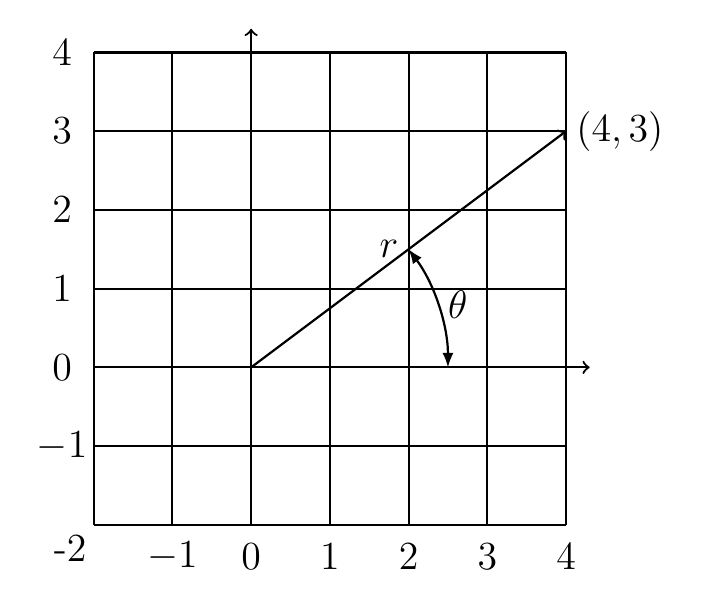
\begin{tikzpicture}[thick,font=\Large]
		\draw[step=1.0,black,thick] (-2,-2) grid (4, 4);
		\foreach \i in {-1, ..., 4} {
			\node[align=left] at (\i, -2.4) {$\i$};
			\node[align=left] at (-2.4, \i) {$\i$};
		}
		\node at (-2.3, -2.3) {-2};
		%% Axis
		\draw[->] (4, 0) -- (4.3, 0);
		\draw[->] (0, 4) -- (0, 4.3);
		%% else
		\draw[thick, ->] (0, 0) -- (4, 3) node [midway, left] {$r$} node [right] {$(4, 3)$};
		\draw[latex-latex]  (0:2.5) arc (0:36.87:2.5) node[midway, right]{$\theta$};
	\end{tikzpicture}
	}
	\caption{Coordenadas cartesianas e polares.}
\end{figure}
	
	O ponto $(4, 3)$, quando escrito em coordenadas polares, nos dá:
	\begin{align*}
	r &= \sqrt{4^2 + 3^2} = \sqrt{16 + 9} = \sqrt{25} = 5\\
	\theta &= \arctan\frac{3}{4} = 0.6435 \text{ rad} \approx 36.87^{\circ}
	\end{align*}
	
	\quest{} Construa duas funções: \texttt{polar(x, y)} levará um ponto em coordenadas cartesianas $(x, y)$ para a forma polar $(r, \theta)$ e \texttt{cart(r, theta)}, que fará o caminho contrário.\\
	
	\clue{} O módulo \texttt{math} contém as funções trigonométricas \texttt{math.sin}, \texttt{math.cos} e \texttt{math.tan}, assim como as inversas \texttt{math.asin}, \texttt{math.acos} e \texttt{math.atan}. Para a raiz quadrada, você pode usar a função \texttt{math.sqrt}.\\
	
	\example
	\begin{lstlisting}
>>> import math
>>> polar(-1, 0)
(1.0, 3.141592653589793)
>>> cart(2, math.pi)
(-2.0, 0.0)
	\end{lstlisting}
	
	\pagebreak
	
	\problem[0]{Números de Fibonacci e a proporção áurea}

	A proporção áurea, muitas vezes representada pela letra grega $\varphi$ (phi), ficou conhecida ainda na grécia antiga por representar um padrão de beleza estética. Sua presença se mostrou marcante também na construção artística renascentista e se encontra até hoje em objetos do cotidiano como nas telas de celulares e nos cartões de crédito.
	
	\begin{figure}[H]
\centering
% I have seen many beautiful depictions of Fibonacci spirals and
% golden spirals. So I thought it would be nice to make a Fibonacci
% spiral in TikZ. I like the look of white on black so here I define a
% black background rectangle.
\resizebox{200pt}{!}{%
\begin{tikzpicture}[background rectangle/.style={fill=white},
                    show background rectangle] 
  % Create some counters for holding the Fibonacci numbers
  \newcounter{a}
  \newcounter{b}
  \newcounter{temp}

  % Initialize the counters
  \setcounter{a}{0}
  \setcounter{b}{1}

  % The spiral will start at the origin
  \coordinate (0) at (0,0);

  % This loop defines the number of turns in the spiral. Note that we
  % will have to be careful not to overflow our counters or make the
  % spiral too large for TeX to handle. This is easy to do as the
  % Fibonacci sequence grows exponentially.
  \foreach \i in {1,...,18}
  {
    % Get the "name" of the last point on the spiral
    \pgfmathsetmacro{\lastpoint}{\i-1}

    % Compute the angle for this turn of the spiral
    \pgfmathsetmacro{\startangle}{mod(\i-1,4) * 90}

    % Draw this turn of the spiral and remember the point where we end 
    \draw[black] (\lastpoint) arc 
      (\startangle : \startangle + 90 : \value{b}/10.0pt) coordinate (\i);

   % Compute the next Fibonacci number
    \setcounter{temp}{\value{b}}
    \addtocounter{b}{\value{a}}
    \setcounter{a}{\value{temp}}
 }

 % Add some framing for the spiral while at the same time not "boxing"
 % it in. Note that to put a square around each turn of the spiral we
 % could have just used the command \draw[white] (\lastpoint)
 % rectangle (\i); after drawing each turn in the loop above.
 \foreach \i in {1,3,...,17}
 {
   \pgfmathsetmacro{\lastpoint}{\i-1}
   \draw[black] (\lastpoint) -| (\i);
 }

 \foreach \i in {2,4,...,16}
 {
   \pgfmathsetmacro{\lastpoint}{\i-1}
   \draw[black] (\lastpoint) |- (\i);
 }

 \draw[black] (17) -- (17 |- 18);
 
 \draw[black] (18) -- +(14.7, 0) -- +(14.7, 9.1) -- +(0, 9.1) -- (18);
\end{tikzpicture}
}
\caption{Espiral de Fibonacci}
\end{figure}
	
	A constante numérica que representa a razão áurea está intimamente ligada a uma sequência de números também há muito conhecida:
	$$0, 1, 1, 2, 3, 5, 8, 13, 21, 34, ...$$
	Esta sequência foi descoberta por Fibonacci enquanto estudava a reprodução dos coelhos. Depois disso, padrões dessa forma foram encontrados em vários outros processos da natureza, desde a forma dos girassóis até as ramificações das algas marinhas. A sequência começa com o 0 e o 1. Para calcular qualquer outro número, basta somar os seus dois antecessores. A proporção áurea, por sua vez, é aproximada pela razão entre dois números de Fibonacci consecutivos:
	$$\varphi \approx \frac{F_{i+1}}{F_{i}}$$
	A aproximação fica melhor conforme os números escolhidos se tornam maiores.\\
	
	\quest Faça uma função que calcule o $n$-ésimo número de Fibonacci. Em seguida use a função que você criou para calcular uma aproximação da razão áurea.
	
	
	
	\pagebreak
	
	\section{Aula II - Condicionais \\(\stmt{if}, \stmt{elif}, \stmt{else}, \type{bool}, \stmt{True}, \stmt{False})}
	
	\problem[0]{Dentro do círculo\label{sec:2.1}}
	
	O círculo unitário é aquele que tem raio $1$ e se encontra centrado na origem $(0, 0)$ do plano cartesiano.
	
	\begin{figure}[H]
	\centering
	\resizebox{200pt}{!}{%
	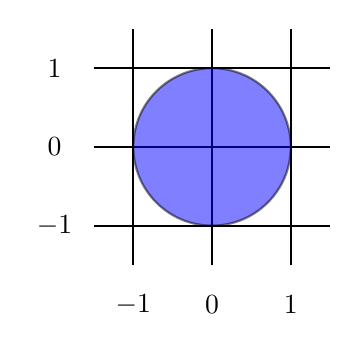
\begin{tikzpicture}[thick]
		\draw[step=1.0,black,thick] (-1.5,-1.5) grid (1.5, 1.5);
		\foreach \i in {-1, ..., 1} {
			\node[align=left] at (\i, -2) {$\i$};
			\node[align=left] at (-2, \i) {$\i$};
		}
		\draw[fill=blue, semitransparent] (0,0) circle[radius=1];
	\end{tikzpicture}
	}
	\caption{Círculo Unitário}
\end{figure}
	
	\quest Faça uma função que diga se um ponto $(x, y)$ se encontra dentro ou fora do círculo unitário, retornando \stmt{True} ou \stmt{False} respectivamente.\\
	
	\example
	\begin{lstlisting}
>>> dentro(1, 1)
False
>>> dentro(0, 0)
True
>>> dentro(1, 0)
True
>>> dentro(0.5, 0.5)
True
	\end{lstlisting}
	
	\pagebreak
	
	\problem[0]{Intersecção de Retângulos}
	
	Uma maneira simples de representar retângulos em um computador é através de um par de pontos, onde cada ponto é um par ordenado $(x, y)$. Por convenção, o primeiro ponto indica o canto superior esquerdo do retângulo; e o segundo, o canto inferior direito.\\
	
	\begin{figure}[H]
	\centering
	\begin{tikzpicture}
	\draw[draw=black] (11.1,5.5) rectangle ++(0.3,0.3);
	\end{tikzpicture}
\end{figure}
	
	Assim, o retângulo \textcolor{blue}{\textbf{azul}} pode ser descrito pelos pares $(1, 4)$ e $(5, 2)$, enquanto o retângulo \textcolor{red}{\textbf{vermelho}} é dado pelos pontos $(3, 3)$ e $(6, 1)$. A intersecção entre os dois é justamente a área \textcolor{indigo}{\textbf{lilás}} que se encontra entre os pontos $(3, 3)$ e $(5, 2)$. \\
	
	\quest Fazer uma função que, dados dois retângulos, retorna a intersecção entre eles, ou seja, um outro retângulo ou \stmt{None}, caso não haja sobreposição.\\
	
	\clue Utilize as funções \type{max} e \type{min}.\\
	
	\example
	\begin{lstlisting}
>>> A = (1, 4, 5, 2)
>>> B = (3, 3, 6, 1)
>>> C = intersec(A, B)
>>> print(C)
(3, 3, 5, 2)
	\end{lstlisting}
	
	\pagebreak
	
	\problem[0]{Anos bissextos}
	
	A humanidade sempre teve problemas com a contagem dos anos, uma vez que estes duram 365,24 dias. O calendário Juliano, que vigorou de 45 a.C. até 1582 d.C., introduziu o uso dos anos bissextos acrescentou um dia a cada 3 anos. O erro só foi percebido décadas depois e o acréscimo foi abandonado. Isso fez com que se acumulasse um erro de cerca de 10 dias até o momento da transição para o calendário Gregoriano. Por conta disso, os dias entre 4 e 15 de outubro de 1582 simplesmente não existiram.\\
	
	Com este novo calendário foi definida a nova regra para o cálculo dos anos bissextos:
	
	\begin{itemize}
		\item De 4 em 4 anos é ano bissexto.
		\item De 100 em 100 anos não é ano bissexto.
		\item De 400 em 400 anos é ano bissexto.
		\item Prevalecem as últimas regras sobre as primeiras.
	\end{itemize}
	
	\quest Sabendo que o ano 2000 foi bissexto, crie uma função que, dado um ano, informe se ele é bissexto ou não, retornando \stmt{True} ou \stmt{False}, respectivamente.\\
	
	\example
	\begin{lstlisting}
>>> bissexto(2000)
True
>>> bissexto(2100)
False
>>> bissexto(2104)
True
	\end{lstlisting}
	
	\pagebreak
	
	\problem[0]{Meia-entrada}
	
	A Lei Federal nº 12933/2013, também conhecida como Lei da Meia-Entrada, garante o benefício do pagamento de Meia-Entrada para estudantes, pessoas com deficiência e jovens, de baixa renda, com idade entre 15 e 29 anos. Já a Lei Federal nº 10741/2003, mais conhecida como Estatuto do Idoso, as pessoas com idade igual ou superior a 60 anos tem direito à Meia-Entrada para eventos artísticos e de lazer. Aqui no estado do Rio de Janeiro, contamos ainda com a Lei Estadual RJ n° 3.364/00, que garante o benefício a todos os menores de 21 anos.\\
	
	\quest Escreva a função \texttt{meia\_entrada} que receba os parâmetros \texttt{idade} (\type{int}), \texttt{estudante} (\type{bool}), \texttt{deficiencia} (\type{bool}), \texttt{baixa\_renda} (\type{bool}) e informe com \stmt{True} ou \stmt{False} se a pessoa tem direito ao desconto.\\
	
	\example
	\begin{lstlisting}
>>> meia_entrada(60, False, False, False)
True
>>> meia_entrada(30, True, False False)
False
>>> meia_entrada(20, False, False, False)
True
	\end{lstlisting}
	
	\pagebreak
	
	\section{Aula III - Listas e Loops \\(\stmt{while}, \stmt{for}, \type{list})}
	
	\problem[0]{Sequência de \emph{Collatz}}
	
	A sequência de \emph{Collatz} é obtida aplicando sucessivamente a função
	{\large
		\begin{align*}
		f(n) = \begin{cases}
		3n + 1, &\text{ se } n \text{ for ímpar}\\
		n \div 2, &\text{ se } n \text{ for par}
		\end{cases}
		\end{align*}
	}
	Por exemplo, começamos com $n = 26$. Após sucessivas aplicações temos:
	$$26 \to 13 \to 40 \to 20 \to 10 \to 5 \to 16 \to 8 \to 4 \to 2 \to 1$$
	Isso nos dá uma sequência com $11$ números. $40$ é maior que $26$, mas sua sequência só teria $9$ números.\\
	\\
	Ainda não se sabe se todos os números induzem uma sequência que termina em $1$. No entanto, até agora não foi encontrado um número sequer em que isso não tenha acontecido!\\
	\\
	\quest Faça uma função que calcule o comprimento da sequência gerada a partir de um número natural $n$ qualquer.\\
	
	\example
	\begin{lstlisting}
>>> collatz(26)
11
>>> collatz(40)
9
>>> collatz(1)
1
	\end{lstlisting}
	
	\pagebreak
	
	\problem[0]{Crivo}
	
	O Eratóstenes foi um cara que viveu em 200 a.C., inventou um crivo e calculou a curvatura da terra.
	\figura[height=80pt]{eratostenes.png}{Eratóstenes de Cirene}
	Um \textbf{crivo} é uma forma de saber quem são os números primos até um determinado limite $\mb{N}$. O Crivo de Eratóstenes funciona de forma bem simples:
	
	\begin{enumerate}
		\item Escrevemos em uma tabela todos os números de 0 até $\mb{N}$.

		\item Riscamos o 0 e o 1 e andamos para o 2.

		\item Se um número não estiver riscado, riscamos todos os múltiplos deste, menos o próprio.
		
		\item Andamos para o próximo número e repetimos a etapa anterior (3).		
	\end{enumerate}
	
	Uma maneira interessante de fazer isso é criando uma lista \texttt{L} de tamanho $\mb{N} + 1$, ou seja, cujos índices vão de 0 até $\mb{N}$. Nessa lista, a princípio, supomos que todos os números são primos, então todas as suas entradas serão \stmt{True}. Riscar um número significa transformar uma entrada em \stmt{False}\\
	
	\quest Implemente o crivo de Eratóstenes, retornando uma lista com os números primos entre 0 e $\mb{N}$.\\
	
	\example
	\begin{lstlisting}
>>> crivo(10)
[2, 3, 5, 7]
>>> crivo(20)
[2, 3, 5, 7, 11, 13, 17, 19]
	\end{lstlisting}
	
	\pagebreak
	
	\problem[0]{Troco}
	
	Abaixo temos as moedas atualmente em circulação no Brasil. Como não temos mais a moeda de 1 centavo, não é possível dar troco para qualquer quantia. Por exemplo, se um estabelecimento deve R\$ 0,91 de troco a um cliente, este daria 95 centavos de volta, conforme recomenda o PROCON.
	\figura[width=200pt]{moedas.png}{Moedas em circulação no Brasil}
	Quando se trabalha com dinheiro no computador, é comum fazer operações com centavos, e não com o valor usual da moeda. Assim, utiliza-se o tipo \type{int} em vez de usar o \type{float}, que pode trazer problemas de arredondamento.\\
	
	\quest Faça uma função que, dada uma quantia qualquer em centavos, retorne uma lista contendo a quantidade de cada moeda, de maneira a utilizar a menor quantidade de moedas possível.\\
	
	\clue Começe com uma lista contendo os valores das moedas, em centavos.\\
	
	\begin{lstlisting}
moedas = [100, 50, 25, 10, 5]
	\end{lstlisting}	
	~\\
	\example
	\begin{lstlisting}
>>> troco(200)
[2, 0, 0, 0, 0]
>>> troco(91) # aqui daremos 95 centavos de troco!
[0, 1, 1, 2, 0]
	\end{lstlisting}
	\pagebreak
	
	\section{Aula IV - Matrizes e Aleatoriedade}
	
	\problem[0]{Viagem pela Europa}
	
	O jogo Viagem pela Europa\footnote{É um jogo bastante antigo e que não se encontra mais nas lojas. Para se ter uma ideia, no mapa aparece a Alemanha ainda dividida nas porções Ocidental e Oriental.} tem um mapa com diversas cidades ligadas por caminhos. Quando começa, cada jogador recebe uma série de cartas e tem que passar por todas elas, cumprindo o roteiro na ordem que preferir. A cada turno se joga um dado, que diz quantas cidades o jogador pode ir adiante.
	
	\figura[width=200pt]{viagem-pela-europa.png}{Caixa do Jogo Viagem Pela Europa}
	
	Podemos representar o tabuleiro do jogo usando uma matriz $A$ de dimensão $N \times N$, onde $N$ é o número de cidades. Assim, o valor da posição \code{A[i][j]} será 1 caso exista um caminho entre as cidades \code{i} e \code{j}, e 0 no caso contrário.\\
	
	\quest Faça uma função, que dada uma matriz \code{A} representando o tabuleiro, diga se existe uma ligação entre duas cidades, \code{i} e \code{j}, mesmo que passando por outras no percurso.\\

	\example
	\begin{lstlisting}
>>> A = [[ 1, 0, 0, 1, 0],
		 [ 0, 1, 0, 0, 1],
		 [ 0, 0, 1, 0, 1],
		 [ 1, 0, 0, 1, 0],
		 [ 0, 1, 1, 0, 1]]
	\end{lstlisting}
	
	Em um caso simplificado, essa matriz representa o seguinte tabuleiro:
	
	% 
\begin{figure}[H]
\centering
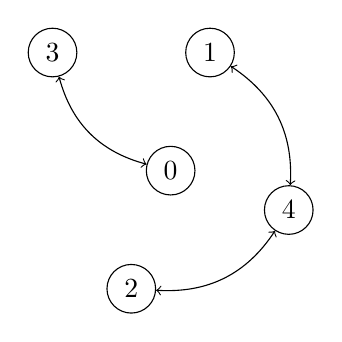
\begin{tikzpicture}
%% Nodes
\node[draw, circle](0) at (2.5, 1.5) {0};
\node[draw, circle](1) at (3, 3) {1};
\node[draw, circle](2) at (2, 0) {2};
\node[draw, circle](4) at (4, 1) {4};
\node[draw, circle](3) at (1, 3) {3};
%% Lines
\draw[bend left ,<->] (0) to node [auto] {} (3);
\draw[bend left ,<->] (1) to node [auto] {} (4);
\draw[bend right,<->] (2) to node [auto] {} (4);
\end{tikzpicture}
\caption{Tabuleiro}
\end{figure}
	
	Dessa forma, teríamos:
	\begin{lstlisting}
>>> tem_caminho(A, 0, 1)
False
>>> tem_caminho(A, 0, 3)
True
>>> tem_caminho(A, 1, 2) # Passando pela cidade `4`
True
	\end{lstlisting}

	\textbf{Desafio Bônus:} Para uma matriz \code{A}, e para um par de cidades \code{i} e \code{j}, faça uma outra função que calcule a menor distância entre as duas, segundo o mapa representado por \code{A}. Quando não houver caminho possível, lembre de retornar \stmt{None}\\
	
	\example
	\begin{lstlisting}
>>> distancia(A, 0, 1)
None
>>> distancia(A, 0, 3)
1
>>> distancia(A, 1, 2) # Passando pela cidade `4`
2
	\end{lstlisting}

	\pagebreak
	
	\problem[0]{Gerando números aleatórios}
	
	Quando pensamos em gerar números aleatórios, temos em mente duas características: Um intervalo de ocorrência desses números e a sua distribuição. Por enquanto, vamos ficar com uma distribuição uniforme, isto é, os números em um intervalo $[a, b]$ tem igual probabilidade de serem gerados.
	
	\begin{figure}[H]
	\centering
	\begin{minipage}{0.45\textwidth}
		\centering
		\scalebox{1.5}{%
			\begin{tikzpicture}
			\draw[->] (-2, 0) -- (2,0) node[right] {$x$};
			\draw[->] (0, 0) -- (0,1.4) node[above] {$y$};			
			\draw[domain=-1:1,smooth,variable=\x,blue] plot ({\x},{1});
			\draw
			\draw[blue] (-1, 0) -- (-1, 1);
			\draw[blue] ( 1, 0) -- ( 1, 1);
			\end{tikzpicture}
			}
		\caption{Distribuição Uniforme}
	\end{minipage}
	\hfill
	\begin{minipage}{0.45\textwidth}
		\centering
		\scalebox{1.5}{%
			\begin{tikzpicture}
			\draw[->] (-2, 0) -- (2,0) node[right] {$x$};
			\draw[->] (0, 0) -- (0,1.4) node[above] {$y$};
			\draw[domain=-2:2,smooth,variable=\x,red] plot ({\x},{exp(-\x*\x)});
			\end{tikzpicture}
			}
		\caption{Distribuição Normal}
	\end{minipage}
	\caption{Pontos aleatórios sobre uma região do plano}
\end{figure} 
	
	\pagebreak
	
	\problem[0]{Calculando $\pi$}
	
	Uma maneira, dentre muitas outras, de se calcular a área qualquer de uma região do plano é conhecida como Método de Monte Carlo. Esta técnica já é amplamente conhecida e seu estudo já se tornou bastante sofisticado. Mesmo assim, sua ideia fundamental pode ser compreendida facilmente.\\
	
	Temos uma região sombreada (em \textbf{\textcolor{blue}{azul}}) e queremos saber sua área. Sorteamos então 20 pontos aleatoriamente dentro do quadrado $6 \times 6$ que envolve a figura.
	
	\newcommand{\makeregion}{
\draw [cyan, fill=blue] plot [smooth] coordinates 
{(0, 2.2) (1.5, 2) (0.5, 0.5) (2, 0) (2.5, -0.5) (1, -1.5) (0, -1) (-1, -0.5) (-2, -1) (-2.5, 0) (-1.5, 0.5) (-0.75, 0.75) (-0.5, 1.5) (-0.75, 2) (0, 2.2)};
}
\begin{figure}[H]
	\centering
	\begin{minipage}{0.45\textwidth}
		\centering
		\scalebox{0.8}{
		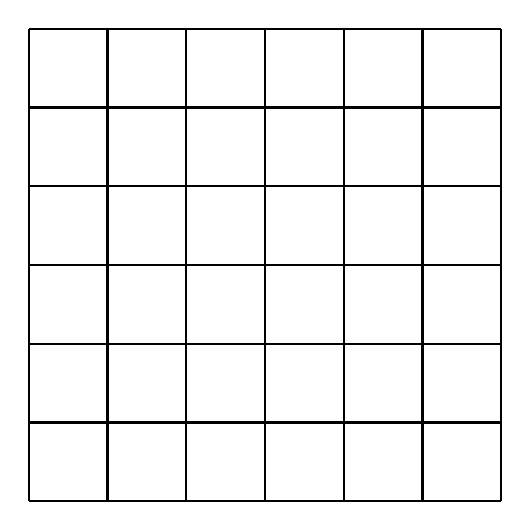
\begin{tikzpicture}
		\makeregion
		\draw [step=1.0,black,thick] (-3,-3) grid (3, 3);
		\end{tikzpicture}
		}
	\end{minipage}
	\hfill
	\begin{minipage}{0.45\textwidth}
		\centering
		\scalebox{0.8}{
		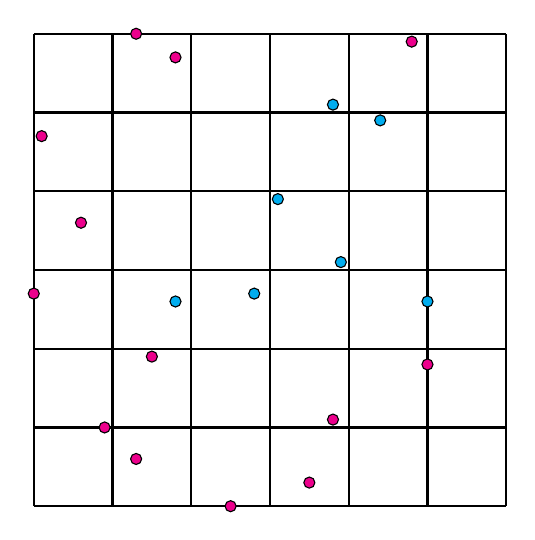
\begin{tikzpicture}
		\makeregion
		\draw [step=1.0,black,thick] (-3,-3) grid (3, 3);
		%% Points
		\draw[fill=magenta] (-0.5, -3.0) circle (2pt);
		\draw[fill=magenta] (-2.9, 1.7) circle (2pt);
		\draw[fill=magenta] (0.5, -2.7) circle (2pt);
		\draw[fill=magenta] (-1.2, 2.7) circle (2pt);
		\draw[fill=magenta] (-1.7, -2.4) circle (2pt);
		\draw[fill=magenta] (-3.0, -0.3) circle (2pt);
		\draw[fill=cyan] (0.1, 0.9) circle (2pt);
		\draw[fill=cyan] (1.4, 1.9) circle (2pt);
		\draw[fill=cyan] (0.9, 0.1) circle (2pt);
		\draw[fill=magenta] (2.0, -1.2) circle (2pt);
		\draw[fill=magenta] (-1.5, -1.1) circle (2pt);
		\draw[fill=cyan] (2.0, -0.4) circle (2pt);
		\draw[fill=magenta] (0.8, -1.9) circle (2pt);
		\draw[fill=magenta] (-1.7, 3.0) circle (2pt);
		\draw[fill=cyan] (0.8, 2.1) circle (2pt);
		\draw[fill=magenta] (-2.4, 0.6) circle (2pt);
		\draw[fill=cyan] (-0.2, -0.3) circle (2pt);
		\draw[fill=magenta] (1.8, 2.9) circle (2pt);
		\draw[fill=cyan] (-1.2, -0.4) circle (2pt);
		\draw[fill=magenta] (-2.1, -2.0) circle (2pt);
		\end{tikzpicture}
		}
	\end{minipage}
\end{figure}
	
	Estão coloridos em \textbf{\textcolor{cyan}{ciano}} os pontos que caíram dentro da região e temos em \textbf{\textcolor{magenta}{magenta}} aqueles que ficaram do lado de fora. Podemos então dizer que a razão entre os pontos que caíram dentro e o total sorteado se aproxima da razão entre a área hachurada e a área do quadrado. Isso nos dá uma fórmula para aproximar a área que desejamos calcular:
	
	$$\text{Área}_{\resizebox{12pt}{!}{\begin{tikzpicture}\makeregion\end{tikzpicture}}} \approx \text{Área}_{\square} \times \frac{\text{\textbf{\textcolor{cyan}{dentro}}}}{\text{\textbf{\textcolor{cyan}{dentro}}} + \text{\textbf{\textcolor{magenta}{fora}}}}$$
	
	\quest Agora pense no caso de um círculo de raio 1 inscrito em um quadrado $2 \times 2$. Utilize a técnica acima para calcular a sua área, que pode ser usada para obter uma aproximação do número $\pi$. Quanto mais pontos sortearmos, melhor será a aproximação.\\
	
	\clue Relembre o exercício\bref{sec:2.1} em que você dizia se um ponto pertencia ou não ao interior de um círculo unitário.
	
\end{document}